%!TEX root = ../template.tex
%%%%%%%%%%%%%%%%%%%%%%%%%%%%%%%%%%%%%%%%%%%%%%%%%%%%%%%%%%%%%%%%%%%%
%% chapter3.tex
%% NOVA thesis document file
%%
%% Chapter with a short latex tutorial and examples
%%%%%%%%%%%%%%%%%%%%%%%%%%%%%%%%%%%%%%%%%%%%%%%%%%%%%%%%%%%%%%%%%%%%

\typeout{NT FILE chapter3.tex}%

\chapter{IVML Designer (A ser implementado)}
\label{cha:ivml_designer}

Como foi abordado no capítulo \ref{cha:introducao}, as ferramentas de análise e desenho de \textit{dashboards} não suportam devidamente o processo iterativo de \textit{design} das mesmas. No presente capítulo, iremos fazer a introdução ao desenvolvimento de uma ferramenta baseada na linguagem \gls{IVML}, com o principal objetivo de culmatar a lacuna presente nas ferramentas mais utilizadas neste âmbito.

Neste capítulo irá ser apresentado o meta-modelo desenvolvido. Este meta-modelo abrange não só a especificação da linguagem \gls{IVML} como toda a metodologia de suporte para a criação de \textit{dashboards}. De seguida, iram ser mencionados os protótipos de solução desenvolvidos, terminando pela listagem de requisitos e tecnologias que a solução desenvolvida necessita de ter presente.

\section{Meta-modelo} % (fold)
\label{sec:meta_modelo}

%Especiificação do meta-modelo em detalhe
%No inicio falar sobre o metamodelo geral, o contexto e motivação que levaram à criação do meta-modelo
%Depois, criar várias secções que vão representar as diferentes componentes que o meta-modelo tem
Com o principal objetivo de apoiar os \textit{designers} no processo de conceção e prototipagem de \textit{dashboards} interativos, foi desenvolvido um meta-modelo que representa de forma estruturada a linguagem IVML e os diversos elementos envolvidos no processo de criação de \textit{dashboards}. Este meta-modelo irá ser utilizado como uma base conceptual para a ferramenta proposta, permitindo a representação tanto das componentes visuais e interativas de um \textit{dashbaord}, como as suas componentes analíticas que sustentam a sua construção.

O desenho e estrutura do meta-modelo foi pensado para englobar não só os elementos visuais utilizados nas representações, como visualizações, interações, e \textit{tooltips}, mas também para incluir as fases iniciais que suportam o processo de criação de \textit{dashboards}, como a definição do âmbito de análise, a formulação de questões analíticas, e a identificação das perspetivas e objetivos de análise. Esta abordagem mais abrangente de elementos tem como objetivo mostrar que o processo de \textit{design} de \textit{dashbaords} interativos não se foca apenas na representação gráfica dos seus elementos, mas também na definição da componente analítica que justifica a sua criação.

É apresentado em apêndice o meta-modelo completo, que englaba todas as diferentes componentes numa só representação (ver apêndice \ref{app:meta_modelo_app}). Nas secções seguintes, vai ser feita a descrição detalhada das diferentes componentes que definem o meta-modelo. Esta abordagem de separação do meta-modelo em diferentes componentes de menor amplitude facilita não só a sua apresentação, como a sua compreensão para um público-alvo menos experiente na área.

\subsection{\textit{Analytical and Structural Component}} % (fold)
\label{sub:anal_struct_comp}

Nesta secção iram ser exploradas em detalhe as duas componentes centrais que definem o meta-modelo, a componente analítica e a componente estrural. A estruturação destas componentes pode ser observada na figura \ref{fig:comp_anal_struct}.

%falar em detalhe sobre as diferentes componentes que a comp anal possuiu, metendo em bolt cada uma das componentes
%posso citar o documento de dissertação da milroy para justificar os exemplos
A componente analítica (...)

A componente estrutural (...)

Ligações entre cada componente

\begin{figure}[htbp]
  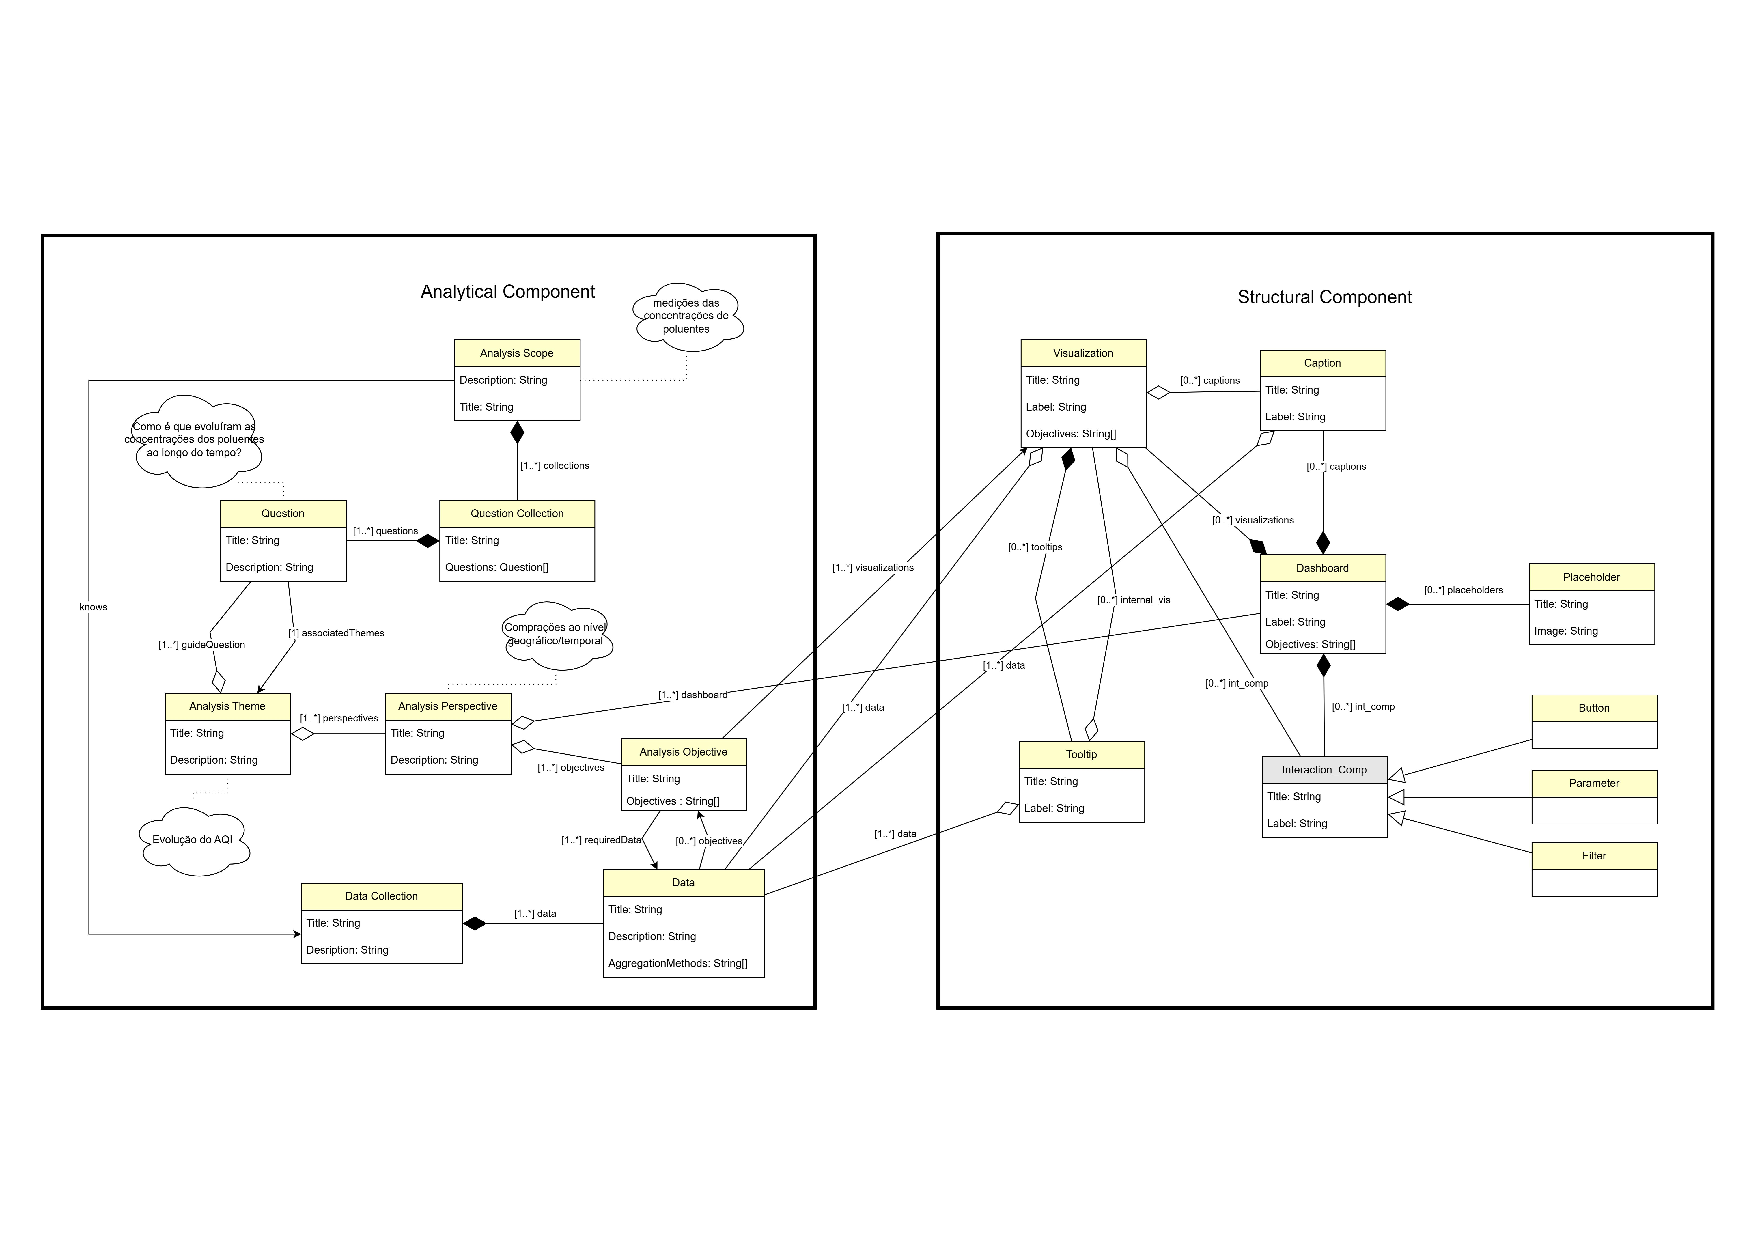
\includegraphics[width=\textwidth]{meta_modelo/compAnlyticalStructural}
  \caption{Componente Analítica e Estrutural do meta-modelo.}
  \label{fig:comp_anal_struct}
\end{figure}

\subsection{\textit{Data and Visual Attributes}} % (fold)
\label{sub:data_vis_attr}

\begin{figure}[htbp]
  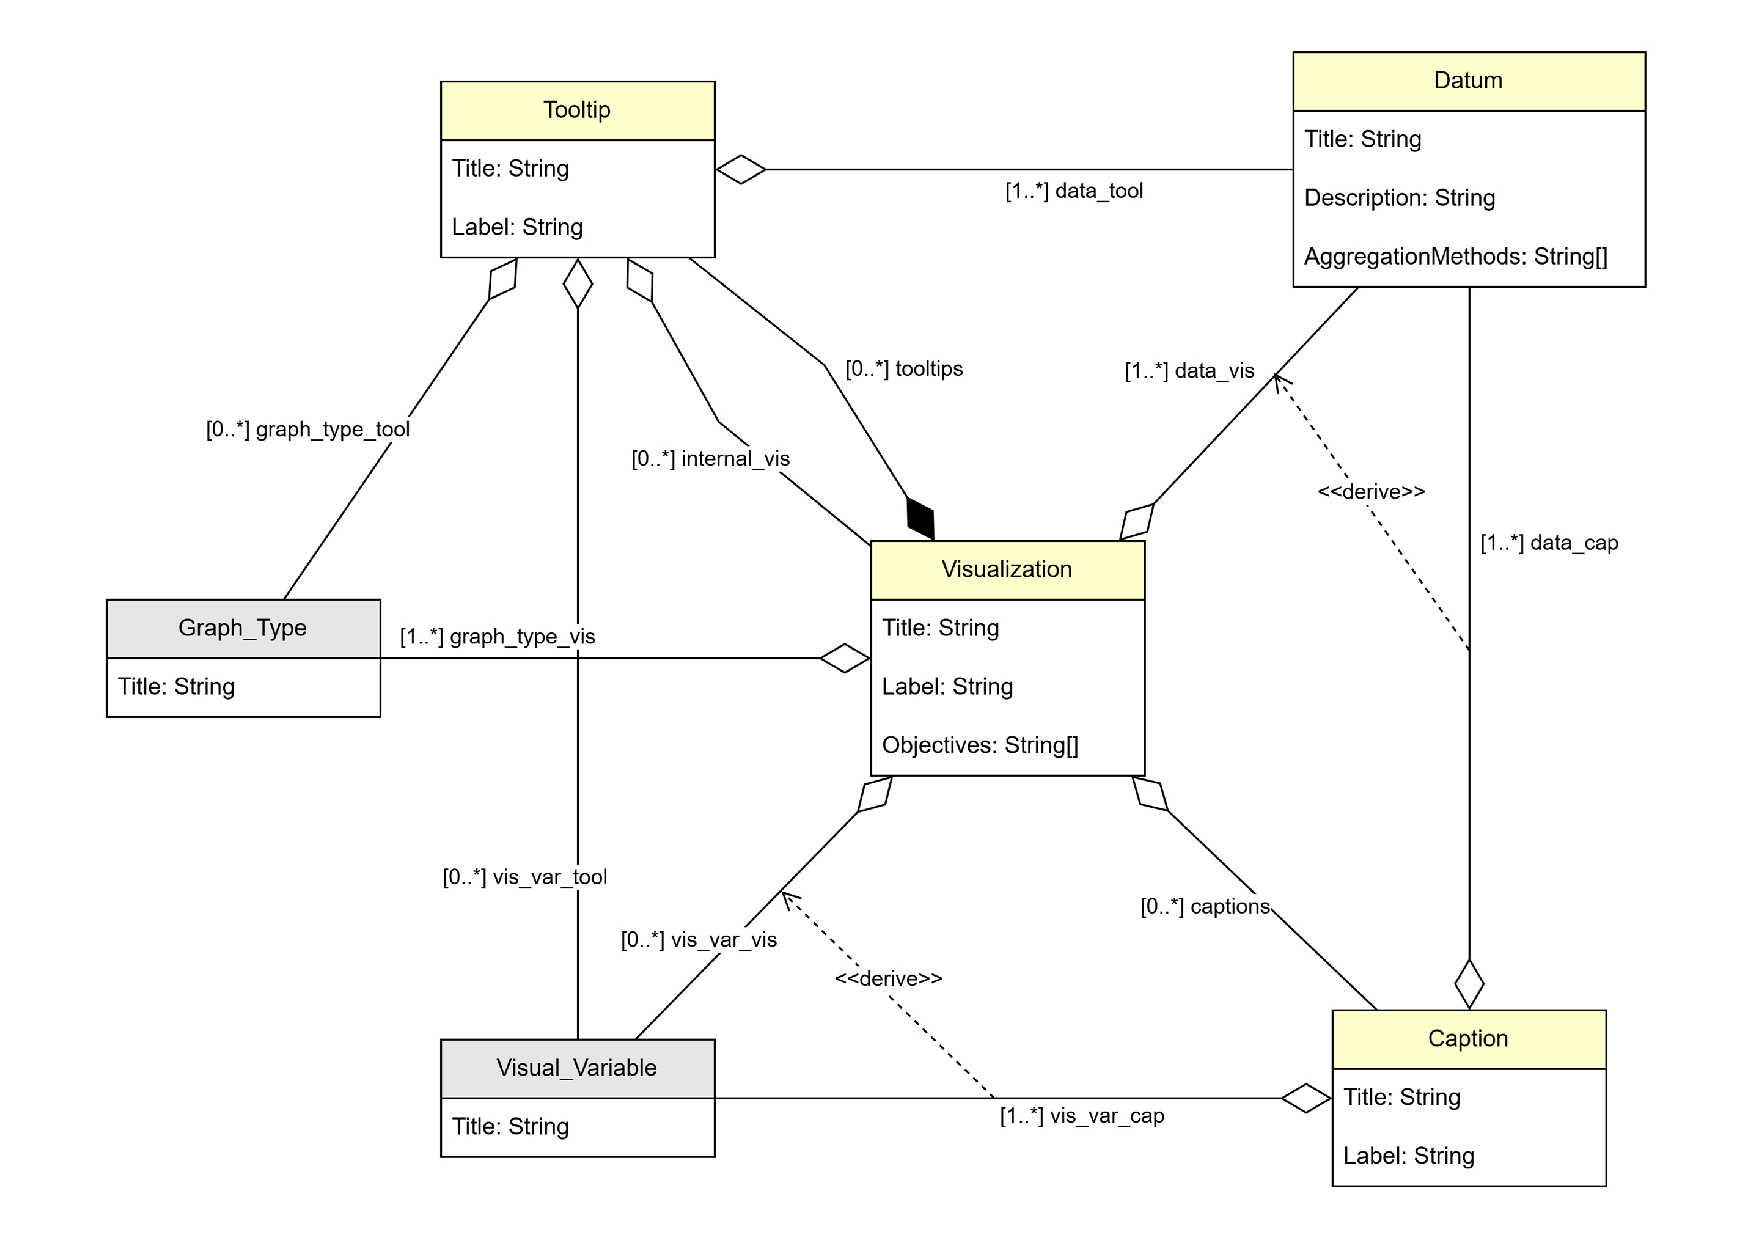
\includegraphics[width=\textwidth]{meta_modelo/dataVis}
  \caption{Componente de Dados e Atríbutos Visuais do meta-modelo.}
  \label{fig:comp_anal_struct}
\end{figure}

\subsection{\textit{Interaction Diagram}} % (fold)
\label{sub:int_diagram}

\begin{figure}[htbp]
  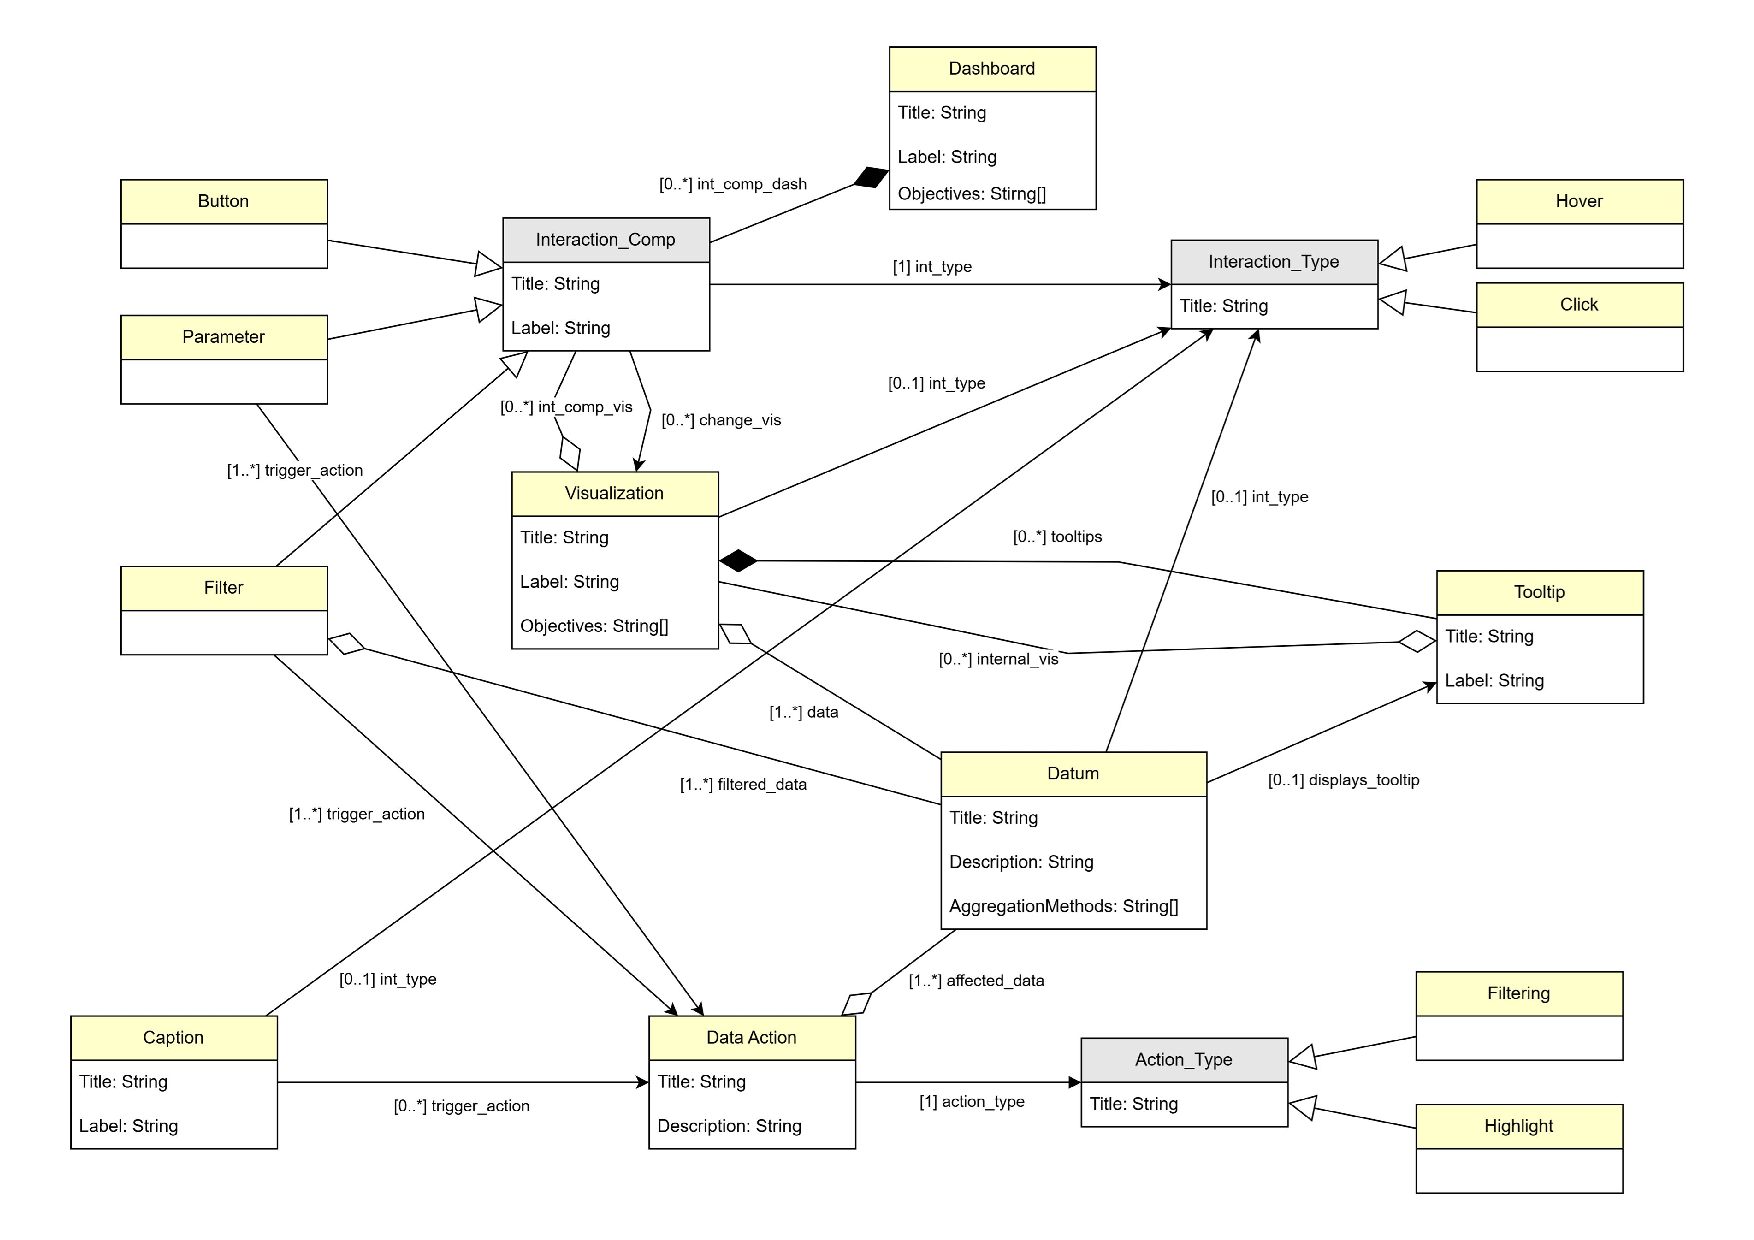
\includegraphics[width=\textwidth]{meta_modelo/interaction}
  \caption{Componente de Interação do meta-modelo.}
  \label{fig:comp_anal_struct}
\end{figure}

\subsection{\textit{Navigation Diagram}} % (fold)
\label{sub:nav_diagram}

\begin{figure}[htbp]
  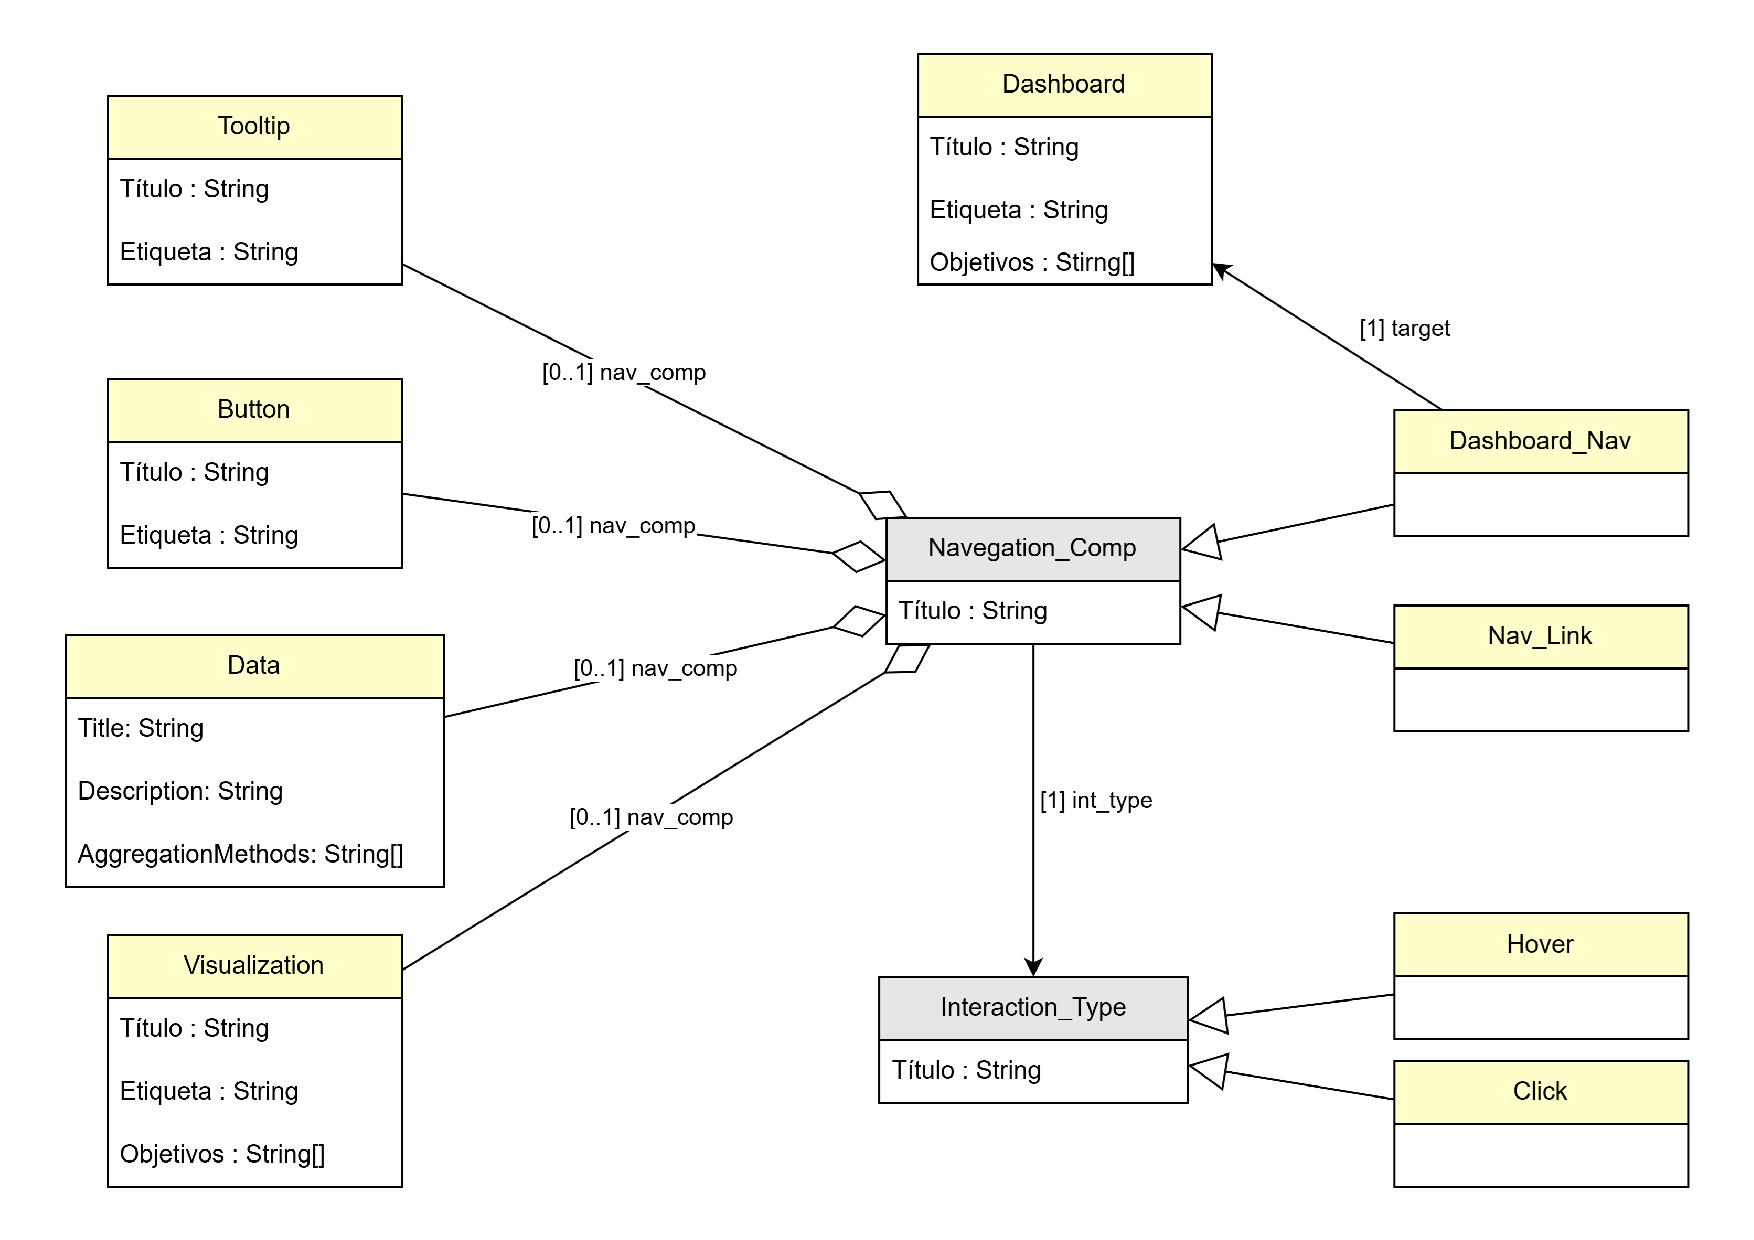
\includegraphics[width=\textwidth]{meta_modelo/navigation}
  \caption{Componente de Vageação do meta-modelo.}
  \label{fig:comp_anal_struct}
\end{figure}

\section{Prototipagem} % (fold)
\label{sec:prototipagem}

%Ver melhor o titulo mas aqui é onde vou falar sobre os prototipos feitos numa fase inicial onde a ferramenta apenas se ia centrar no IVML
%introdução, dizer que meti em anexo o protótipo, dizer que foi numa fase inicial
Para o desenvolvimento de qualquer ferramenta, é crucial que sejam implementados protótipos representativos, quer para representar as diferentes componentes visuais que a mesma terá, quer para representar as componentes técnicas.

Numa fase inicial do desenvolvimento da dissertação, foi implementado um protótipo da ferramenta baseada na linguagem \gls{IVML}. Este protótipo tinha como principal objetivo representar todas as componentes visuais e técnicas que a solução final iria possuir. Uma vez que este protótipo foi realizado numa fase inicial, o mesmo já não se encontra de acordo com a estrutura e organização do meta-modelo desenvolvido e mencionado na secção \ref{sec:meta_modelo}. O protótipo desenvolvido é mostrado no apêndice \ref{}. Como é possível observar, o mesmo apenas representa as diferentes componentes que a linguagem \gls{IVML} possuiu, ignorando toda a componente analítica que é necessária para a criação de diferentes \textit{dashboards} interativas.

\section{Requisitos da ferramenta} % (fold)
\label{sec:requisitos}

%Tecnologias e requisitos que eu já sei que a ferramenta terá de ter
Para tornar a a ferramenta orientada às necessidades dos seus utilizadores, é necessário ter em consideração certas tecnologias para tornar esta experiência o mais orientada para o seu público-alvo. O objetivo principal da criação de uma ferramenta no contexto da dissertação, é auxiliar o processo de conceção e \textit{design} de \textit{dashboards} e facilitar o processo iterativo de comunicação entre os \textit{designer} e \textit{stakeholders}.

De forma a tornar esta ferramenta orientada para as funcionalidades que tem de realizarm, existem algumas características que se tornam imperativas de serem implementadas. Estas característica são:

\begin{itemize}
  \item O utilizador deve estar sempre no controlo.
  \item A interface deve fazer com que os utilizadores tenham um esforço cognitivo mínimo.
  \item A interface deve ser o mais consistente possível.
\end{itemize}


